\section{Slagterieksempel}

\inline{eks1: grise på bånd, foto af flere grise, ingen deadline på kniven. Billeder lægges i kø til kniven som bruger dem hvis de er klar.}

Det første eksempel på en applikation der kan bruge et RTP systemer, er en beslutningsmodel til udskæring af svin.

Vi forestiller os at der findes slagteri hvor  hvert svin skal skæres ud i et forud defineret antal portioner. Til dette bruges en udskæringsrobot og en udskæringsmodel. Udskæringsmodellen er lavet for at minimere mængden af kød der går til spilde.  Det har dog vist sig at udskæringsmodellen ikke altid resultere i en  optimal udskæring af svinet, da  ca. 10\% af alle svin har et ekstra sæt ribben, som modellen ikke tager højde for. Til at løse dette problem har slagteriet udviklet en ny udskæringsmodel for svin med et ekstra sæt ribben, samt  investeret i en røngentskanner der skal skanne alle svin. 
Slagteriet har placeret røngtenskanneren i starten af et transportbåndet mens udskæringsrobotten findes i den anden enden. Der kan være flere svin på transportbåndet på samme tid, og det fremføre svinene i et fast tempo. Dette giver et fast tidsrum fra svinet passere røntgenskanneren til det passere udskæringsrobotten. Vi har hermed et klassisk RTP system, hvor robotten skal foretage et valg af udskæringsmodel under en hard deadline, da det ikke er en mulighed ikke at foretage en udskæring.

Til at understøtte udvælgelsen af model må vi først se arbejdsgangen der er involveret i valget af udskæringsmodel. 
\begin{enumerate}
\tightlist
	\item Et billede bliver taget af svinet mens den passere røntgenskanneren.
	\item Billedet konverteres til en 3D-model af svinet.
	\item 3D-modellen analyseres.
	\item Udskæringmodel udvælges på baggrund af analysen.
	\item Robotten udskærer svinet.
\end{enumerate}

Man kan se at arbejdsgangen indeholder en  række klart afgrænsede arbejdsområder, som med fordel kan modelleres som selvstændige processer i \pycsp. Der findes do ikke kun en måde at opbygge procesnetværket på, men vi har valgt at have følgende processer: Røntgenskanner, Billedekonvertering, 3D-analyse og en udvælgelse og udskæringsproces, hvilket leder til et procesnetværk som vist i \cref{fig:pig-network}.

\begin{figure}
 \begin{center}
  
\includegraphics[scale=1]{images/pig-network}
	\caption{Procesnetværk til udskæring af svin på et slagteri.}
	\label{fig:pig-network}
\end{center}
\end{figure}

Den simple model, viser dog ikke den store fordel, ved RTP systemet i \pycsp, som er at netværket nemt kan udvide antallet af processer til at passe det endelige opstilling. Som programmør har man mulighed for at teste forskellige indstillinger i netværket, som hvor mange processer der samtidigt skal konverterer billederne og hvor mange analyser skal kunne foregå samtidigt. Endeligt kan systemet også nemt udvides hvis det overordnede design på slagteriet ændre sig. Viser det sig f.eks at røntgenskanneren holder netværket tilbage kan man blot udvide procesnetværket med endnu en røngtenproces.

\subsubsection*{Implementering i Greenletsversionen}
Til at implementere eksemplet uden brug af af RTP-udvidelsen i \pycsp, kan vi oprette hvert svin som et objekt og tilknytte en deadline. Nu kan hver proces evaluere om svinet har overskredet sin deadline, i det tilfælde fjerne svinet, og stoppe den videre behandling. Det er ikke angivet hvordan hele processen startes, men vi antager der findes en form for detektor foran røngtenkameraet, der opfanger når et svin passere og som dermed  starter processen. 
Når detektoren starter hele processen, opretter den svineobjektet som den sender til Røngtenprocessen, samt sender en kopi direkte til udvælgelse og udskæringsprocessen. dermed ved processen at der ankommer et svin som den skal udskære, og hvis den inden deadline får en analyse af svinet, kan den træffe et begrundet valg om hvilken model der skal bruges,  men hvis ikke denne analyse findes, bruges blot standardmodellen. \CRef{fig:pig-network2} viser det endelige  netværk, hvor detektoren er introduceret, og som sender data til hhv. Røntgenprocessen og til Udvælgelse og udskæringsprocessen. 

\begin{figure}
 \begin{center}
  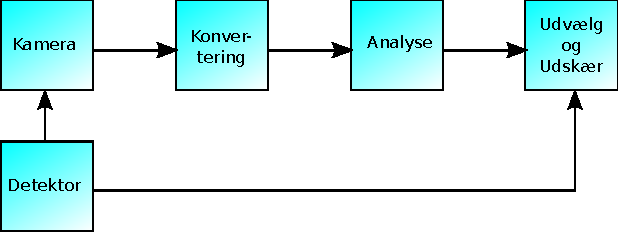
\includegraphics[scale=1]{images/pig-network2}
	\caption{Procesnetværk med detektor til initiering af hvert svin.}
	\label{fig:pig-network2}
\end{center}
\end{figure}

Et problem ved at implementere hele slagterieksemplet i en version bygget på greenletsversionen, er at kun en proces kan være aktiv af gangen. Mens udskæringsprocessen venter på at svinet kommer tæt nok på arbejder konvertering og analyse processen. De skal frivilligt afgive kontrollen, mens svinet er indenfor rækkevidden af robotten, og hvis de ikke gør er udskæringsrobotten låst og  foretager  ikke udskæringen.



%\subsection{Eksempel 2 - Sensornetværk med høj/lav -prioritet}
%\inline{eks2: skal vise alternation, kan være en sensor som modtager måledata med lav prioritet og som skal sende måledata på opdordring med høj prioritet.}
